\chapter{結果}\chaplab{result}
本章では,\chapref{methods}で述べた推定の結果を,最尤推定の結果と比較して議論する.
\section{推定結果のグラフ}
ランダムに分割したテストデータ32個に対し,各時刻に推定を行った結果を,時系列ごとに出力した図が\figref{result_line_error}である.
\begin{figure}[htbp]
  \centering
    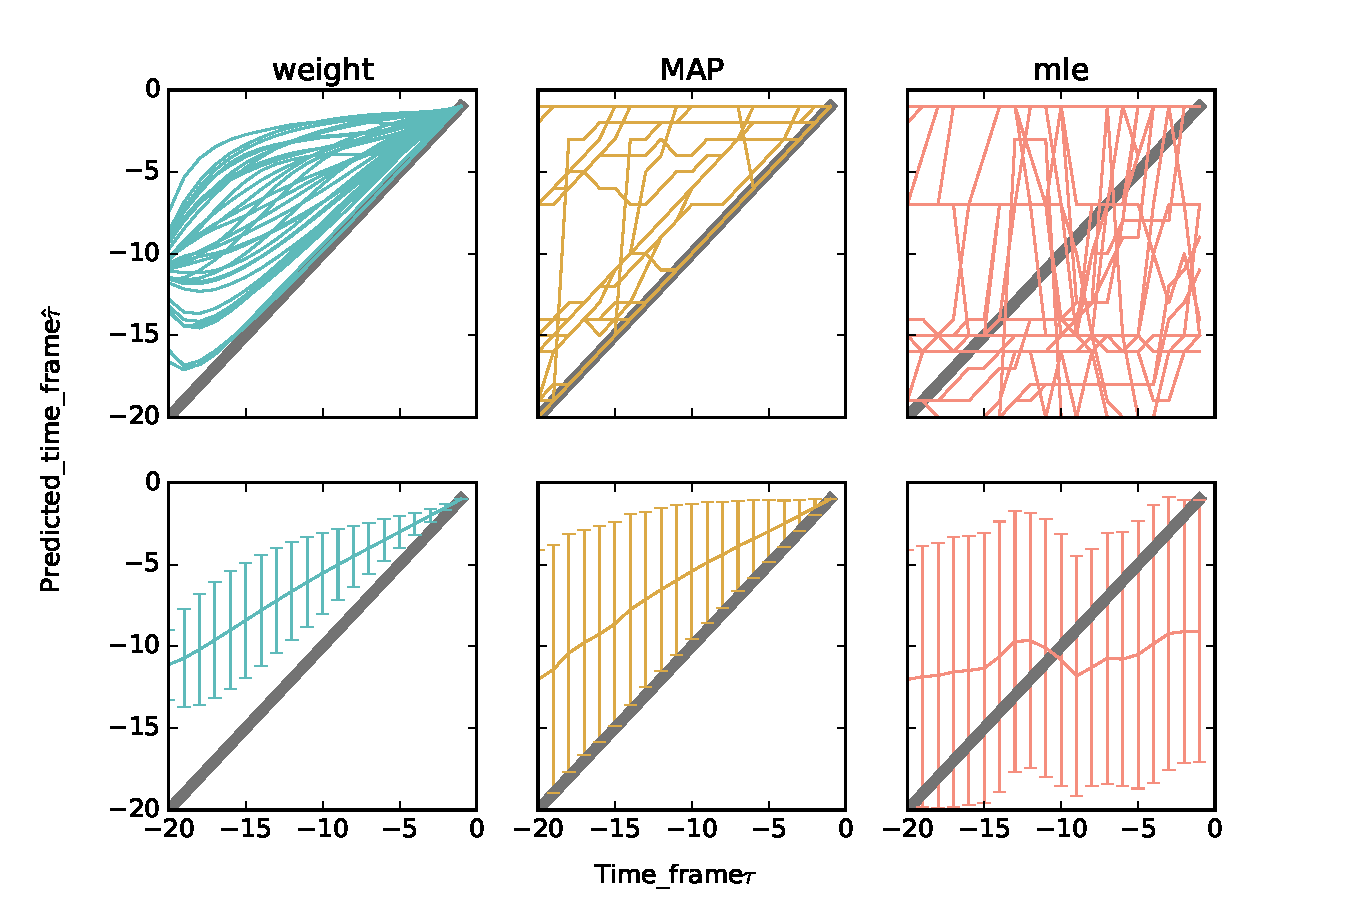
\includegraphics[width=70mm]{fig/result_line_error.pdf}
  \caption{32回の推定結果の推移についての折れ線グラフと,平均,分散をエラーバーで示した図.左から順に,重み付き平均,MAP推定,最尤推定の結果となっている.x軸が実際の時間,y軸が推定時間となっており,実際の時間と推定時間が一致する点を灰色の棒線で繋いでいる.}
  \label{fig:result_line_error}
\end{figure}

左に示した,水色のグラフは,重み付き平均による推定結果,中央の黄色のグラフは,MAP推定による結果,右のオレンジのグラフは,最尤推定により求めた結果を表している.上の3つの図が,各系列での推定結果の推移を表したもので,下の3つの図が,各試行での平均推定時間の推移と,各時刻における散らばりを分散によって示している.中央の灰色の直線は,推定結果の誤差が0となる線を示している.まず,重み付き平均のときは,他と比べ急激に推定結果は変わらず,徐々に推定結果を変化させて行っていることがわかる.対して,MAP推定では,推定の推移の仕方は概ね以下の傾向に分かれていることがわかる.
\begin{itemize}
	\item 最初から最後まで正確に推定を続けているもの(灰色の線に乗っているもの)
	\item 直前であると推定し続けているもの($\hat{\tau}=-1$に張り付いた水平の線)
	\item 途中から推定結果が改善されるもの
\end{itemize}
また,2つの手法で共通して,エラーバーは徐々に小さくなっており,推定が進むにつれて結果が改善されていっていることが読み取れる.最後に,最尤推定の結果では,全時間帯において推定結果が激しく変動しており,また,平均の推定結果についても非常にばらつきが大きくなってしまっていることがわかる.
\par
重み付き平均において,推定を開始した段階では$\hat{\tau}=-10$付近であるとする推定結果が多く見られるが,これは,推定結果を平均として出す関係上,結果が分布の中心点に引っ張られてしまいやすいという特性が存在しているためである.これは,MAP推定において平均を取ったときにも同様に現れる傾向である.
\par
次に,推定結果の誤差をヒストグラムとして表し,各手法を比較したものが\figref{result_hist}である.
\begin{figure}[htbp]
  \centering
    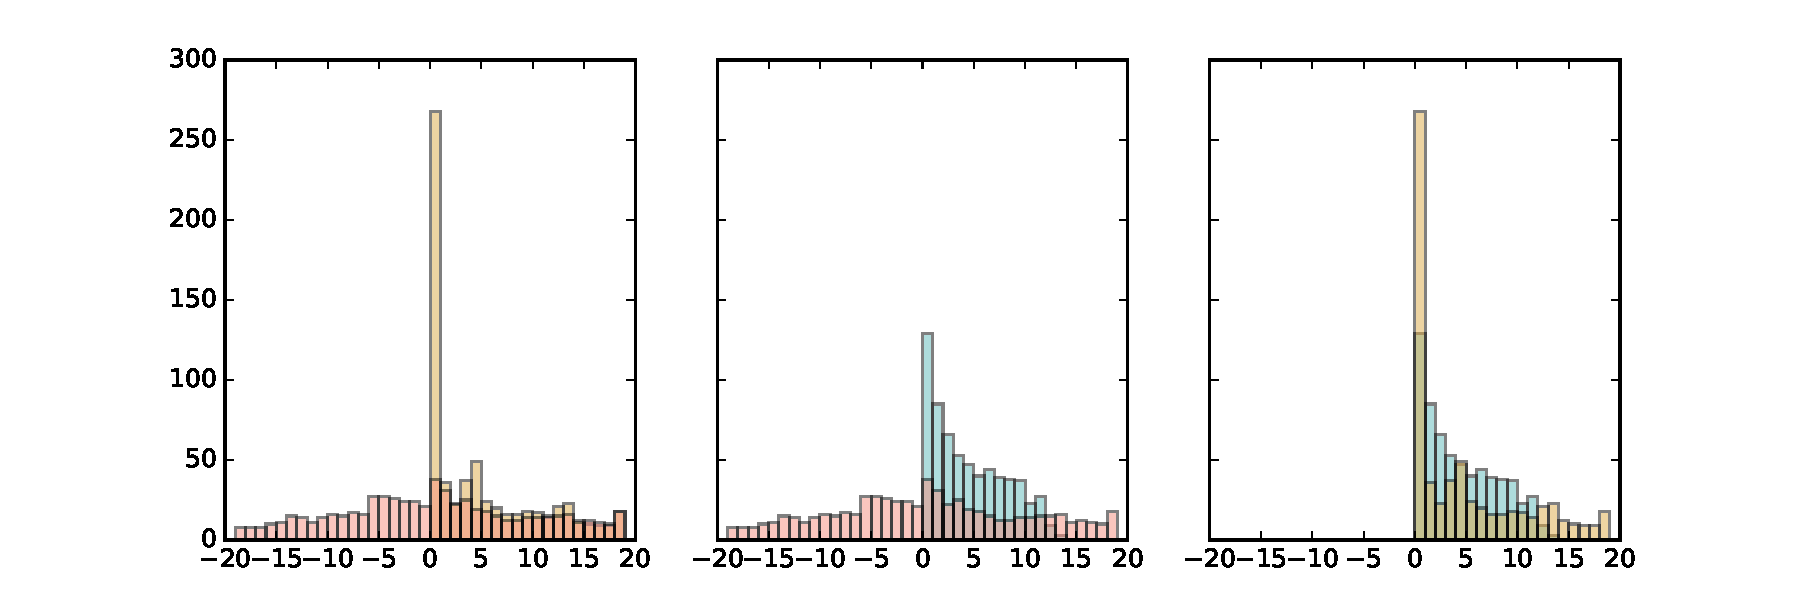
\includegraphics[width=100mm]{fig/result_hist.pdf}
  \caption{32回の推定において得られた誤差をヒストグラムにし,3つの結果をお互いに比較したもの.左から,MAPと最尤推定,最尤推定と重み付き平均,重み付き平均とMAPの比較結果となっている}
  \label{fig:result_hist}
\end{figure}

先程のものと同じく,水色が重み付き平均,黄色がMAP,オレンジが最尤推定である.x軸が誤差,y軸は誤差が出現する頻度を表している.重み付き平均,MAPの両手法とも,最尤推定よりも中心付近,つまり推定誤差が小さいときのの頻度が大きくなっている.特に,MAPは,中心の推定誤差0が際立って大きくなっている.正確な結果を出力する頻度が高いことは,重み付き平均に比べてMAPの利点であると考えられる.しかし逆に,重み付き平均ではほとんど現れない19や20もの誤差が出現する場合がある.これは,最初から最後まで車線変更直前である,と完全に推定を失敗してしまう可能性ががMAPには存在するからである.ある程度の誤差を許容し安定した結果を出したいなら重み付き平均を,完全に失敗するときがあっても,正確に推定することが多いほうが好ましいならMAPを採用するべきだろう.
